\begin{table}[thb] \centering
    \caption{A table with images at the left. Images can be useful to illustrate different setups.} 
    \label{tab:res_synth_mirco_baseline}
    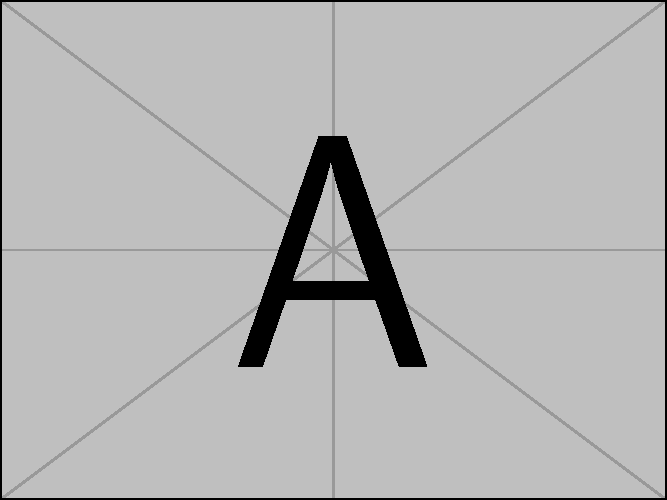
\includegraphics[width=0.088\textwidth,height=0.085\textwidth]{example-image-a}
    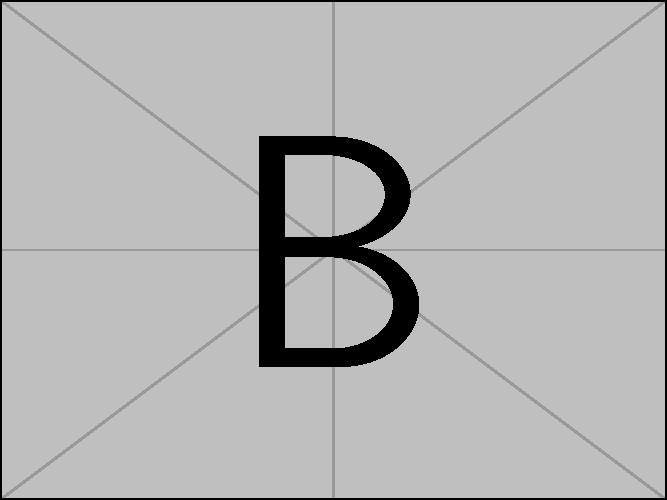
\includegraphics[width=0.088\textwidth,height=0.085\textwidth]{example-image-b}
    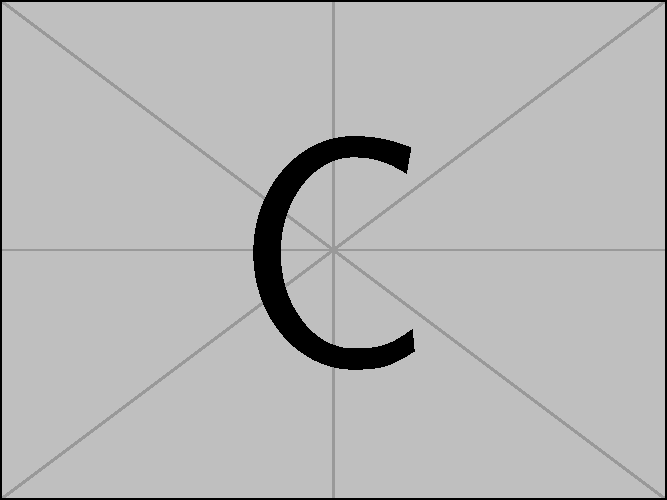
\includegraphics[width=0.088\textwidth,height=0.085\textwidth]{example-image-c}
    \raisebox{0.9\height}{
    \resizebox{0.19\textwidth}{!}{
    \large
    \begin{tabular}{ccc}
        \toprule
        Type & Range & MAE \\
        \midrule
        (a) & 144$\times$144 & 4.21 \\ 
        (b) & 37$\times$37 & 10.90 \\
        (c) & 22$\times$22 & 18.72 \\
        \bottomrule
    \end{tabular}
    }}
    \\
    \vspace{-0.2em}
    \makebox[0.09\textwidth]{\footnotesize (a)} 
    \makebox[0.09\textwidth]{\footnotesize (b)}
    \makebox[0.09\textwidth]{\footnotesize (c)}
    \makebox[0.19\textwidth]{\footnotesize (d) Normal estimation}
    \\
\end{table}
